\subsection{Overview}
\subsubsection{Before Testing}
\begin{itemize}
    \item Test Plan - this document
    \item{Test Cases specification}
\end{itemize}
Here is our test case specification for the tests that are possible from our current development in software. Green = Test has been developed. Blue = Able to be tested.
\begin{figure}[ht!]
\begin{minipage}[t]{0.5\textwidth}
    \centering
    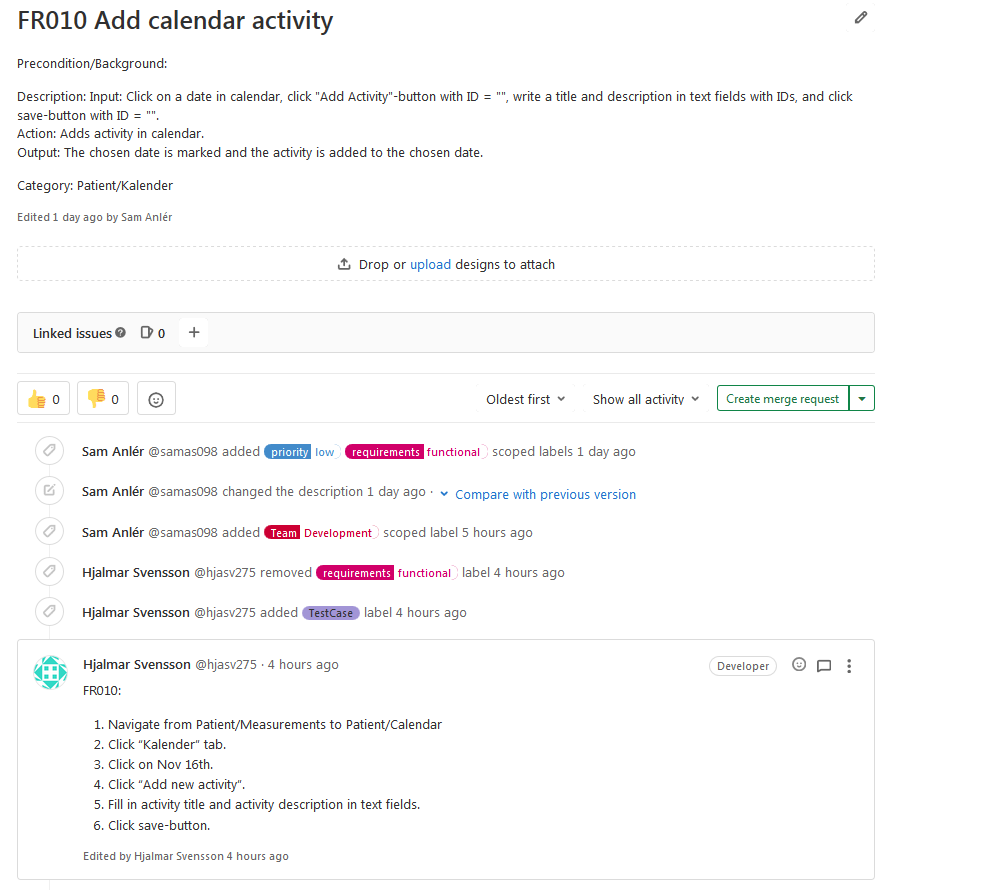
\includegraphics[scale=0.75]{Pictures/TestCase1.PNG}
    \caption{Test Case 1}
\end{minipage}%
\begin{minipage}[t]{0.5\textwidth}
    \centering
    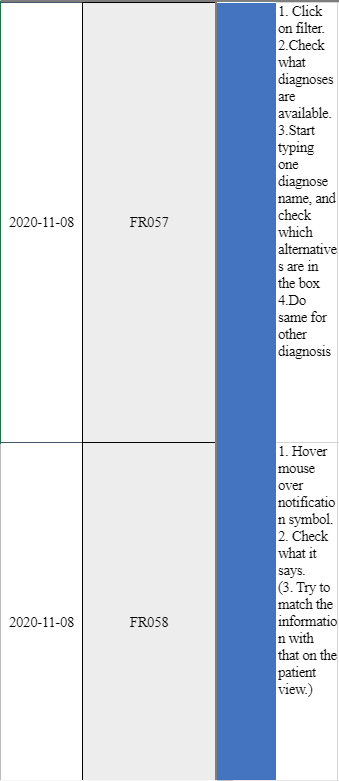
\includegraphics[scale=0.75]{Pictures/TestCase2.PNG}
    \caption{Test Case 2}
\end{minipage}
\end{figure}

\begin{figure}[ht!]
\begin{minipage}[t]{0.5\textwidth}
    \centering
    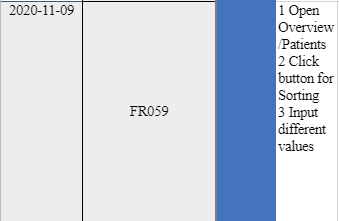
\includegraphics[scale=0.75]{Pictures/TestCase3.PNG}
    \caption{Test Case 3}
\end{minipage}%
\begin{minipage}[t]{0.5\textwidth}
    \centering
    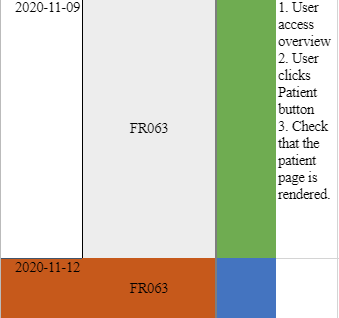
\includegraphics[scale=0.75]{Pictures/TestCase4.PNG}
    \caption{Test Case 4}
\end{minipage}
\end{figure}

\begin{itemize}

    \item{Test Design specification}
    \item{Education Plan}
    \end{itemize}
    In our education plan we have used a Udemy course using JUnit and selenium [3], aswell as watching several youtube videos on selenium and Jest. For the setup of the environment, we have gotten help from our Integrator Emil in setting yarn and npm up. Will be a better write up as a seperate document, will be done in version 3.0.

\subsubsection{During Testing}
\begin{itemize}
    \item Tests
\end{itemize}
For this you can check our RTM that is located in General -> Analysis -> Requirements.xslx . Should map tests to its requirement. For the actual code part of the tests those can be found in the branch testingBranch in the gitlab associated with the project. 
\begin{itemize}
    
    \item{Test Data}
\end{itemize}
Will be added in the RTM together with Test Results.
\begin{itemize}

    \item{Test Traceability}

\end{itemize}
\subsubsection{After Testing}
\begin{itemize}
    \item Test Result
  
\end{itemize}
Will be added in the RTM together with Test Data.
\subsection{Schedule}
\vfill
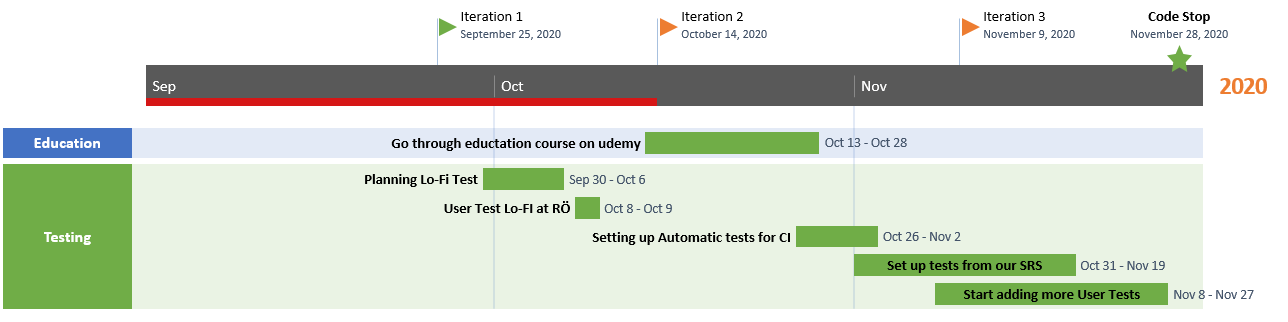
\includegraphics[width=\linewidth]{Pictures/TestSchedule.PNG}

    \vfill
    \clearpage
